%%% -*- TeX-master: "case-study.tex" -*-
\section{Discontinuous Galerkin Methods}
\label{sec:dg}

Discontinuous Galerkin methods (DG) are a class of numerical schemes for solving differential equations that draw on ideas from the finite volume as well as the finite element communities.
For simplicity's sake we will only consider one-dimensional problems.
Consider a spatial domain $X = [a, b] \subset \mathbb{R}$.
Let $u(x, t) : X \times \mathbb{R}_{\ge 0} \rightarrow \mathbb{R}$ be a scalar quantity defined on $X$ that varies with time $t$.
Furthermore consider the partial differential equation
\begin{equation}
  \label{eq:dg-pde}
  u_{t} + f(u)_{x} = 0
\end{equation}
that describes the behavior of $u$ where $u_{t}$ is $u$'s partial derivative with respect to time and $f(u)_{x}$ is the spatial derivative of some function $f$ of $u$.
Now given some boundary conditions, i.e. values for $u(a, t)$ and $u(b, t)$, and initial value conditions $u(x, 0)$ for all $x \in X, t \in \mathbb{R}_{\ge 0}$, we would like to solve Equation \eqref{eq:dg-pde} for $u$.
The first step towards this goal is to discretize the spatial domain -- not necessarily uniformly -- into $n \in \mathbb{N}$ cells $[x_{i}, x_{i + 1}], i \in \{ 0, \dots, n - 1 \}$ such that the cells are ordered ($x_{0} < x_{1} < \dots < x_{n}$) and the resulting mesh covers the domain ($\cup_{i = 0}^{n - 1} [x_{i}, x_{i + 1}] = X$).

DG then approximates the solution $u$ from the data at each point in time $t$ by a piecewise continuous function $U$ that is continuous on the cell interiors but discontinuous at their boundaries.
These $U$ depend on $t$ but since the moment limiter does not work across time steps we will now fix a time $t'$ for the rest of this section and all later mentions of $U$ will mean $U$ at time $t'$.
Written out we have
\begin{equation*}
  U = \bigoplus_{i = 0}^{n - 1} U_{i} \circ \xi_{i}
\end{equation*}
where $\oplus$ is a direct sum, $\circ$ is function composition, $U_{i}$ is a polynomial and $\xi_{i}$ normalizes coordinates in cell $i$ to the reference interval $[-1, 1]$, i.e. $\xi_{i}(x) = 2 \frac{x - x_{i}}{x_{i + 1} - x_{i}} - 1$.
The normalization is required because we employ a special polynomial basis, the \emph{Legendre polynomials}, for the individual $U_{i}$.
So the polynomial on cell $i$ can be written as
\begin{equation*}
  U_{i} = \sum_{j = 0}^{p} c_{i}^{j} P_{j}
\end{equation*}
where $P_{j}$ is the $j$-th Legendre polynomial, $U_{i}$ is of degree $p$ and the $c_{i}^{j}$ are the coefficients that are determined as part of the DG method.

How the solution $U$ is finally used to estimate the derivatives and advance the solution to the next time step goes beyond the scope of this article.
The interested reader is encouraged to refer to \cite[Chapter 3]{Hesthaven2007}.

There are actually two approaches to compute the polynomial approximations called \emph{nodal} and \emph{modal}.
Both find the same approximations in the end but their form makes it so that the modal approach lends itself better to limiting than the nodal approach.
Modal determines the polynomials in the form introduced here and has the advantage that the highest degree portion of the polynomial is solely controlled by the highest non-zero coefficient.
Hence you can decrease the effective order of the polynomial approximation by successively setting the highest coefficient to zero without requiring true $p$-adaptivity in the numerical scheme.
This is necessary to control oscillations in the proximity of discontinuities.

The nodal approach on the other hand uses Lagrange polynomials as basis functions.
These are problematic for limiters insofar that every basis function has degree $p$, so this gradual reduction to lower-order approximations by eliminating the highest-order contributions cannot be realized.
As a consequence the limiters we present are only applicable to modal DG.

Even though the model admits discontinuities at cell boundaries, it develops oscillations in their vicinity nonetheless as discontinuities and steep gradients pass through the cells.
This is demonstrated in Figure \ref{fig:dg-oscillations} where a single shock was simulated for one complete traversal of a cyclic domain.
Such overshoots are not observed in physical processes and therefore stem entirely from numerical errors.

\begin{figure}[h]
  \centering
  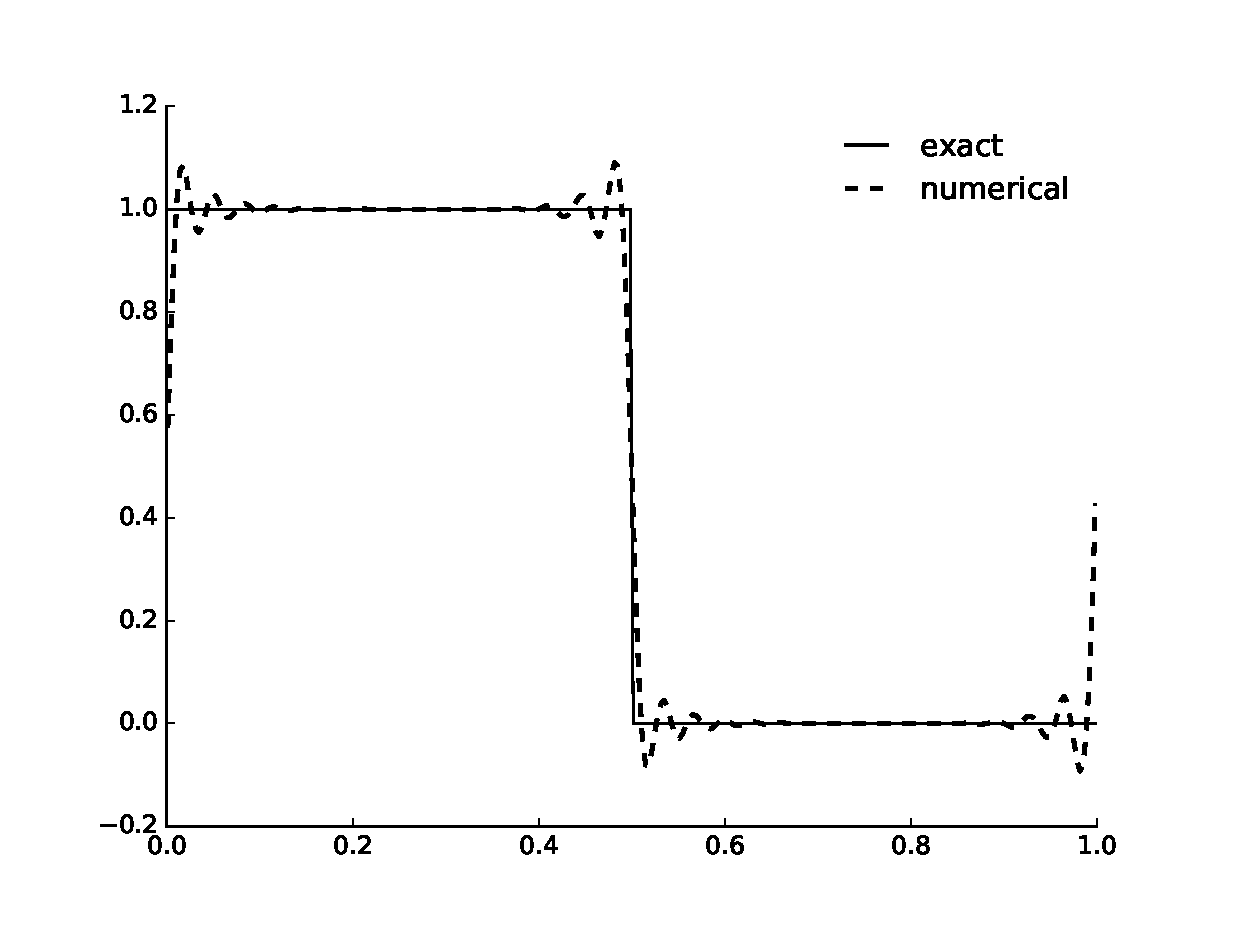
\includegraphics[width=0.8\columnwidth]{figures/oscillations}
  \caption{Linear advection of a shock solved with DG of order $p = 6$ on a grid of $20$ cells. The solution develops oscillations close to the discontinuities.}
  \label{fig:dg-oscillations}
\end{figure}
